\section{Part 1}
\label{sec:part1}

\subsection{Analyzing the results}

\begin{itemize}
	\item Figure 1 is the netplot.png graph that was generated after running the Ping-pong experiment. The minimum time, $\alpha$, to send a message of any size is $4.8532e-05$ s.
	\item When the message size is large, the slope of the line is $8.7719e-09$ s/byte (computed from the results.dat file). This slope represents the extra amount of time required to send every extra byte once the message size exceeds $1000$ bytes. Qualitatively, the slope represents the message-passing latency that is dependent on the bandwidth of the network when the message size is large enough.
	\item To estimate the amount of time, $T(m)$ to send a message of $m$ bytes, we have two cases:
	\begin{enumerate}
		\item when $m < 1000$, $ T(m) = \alpha $ since $\alpha$ is the more prominent term in this case.
		\item when $m > 1000$, $ T(m) = m\beta $ where $\beta = 8.5115e-09$ since the bandwidth of the network is the more prominent term in this case.
	\end{enumerate}
	Combining these two cases, we have the following formula: \\
	\[ T(m) = \alpha + m\beta \]
	\item Line-by-line explanation of the code :
	\begin{enumerate}
		\item lines 1-2: function gets invoked, taking in pointer to the message and its length
		\item lines 3-4: declaring and initializing message tags that will be used for the ping-pong communication
		\item lines 6-7: obtain the id of the process within the MPI\_COMM\_WORLD communicator
		\item line 9: checking if the process is the root (i.e. process 0). If so, lines 10-12 will be executed; otherwise, lines 14-16 will be executed
		\item line 10: declaring an MPI\_Status object
		\item line 11: sends the message of type integer andn length len pointed to by msgbuf to the process 1 in the MPI\_COMM\_WORLD communicator. The process is blocked at this line until the receiving process receives the complete message
		\item line 12: the process is waiting to receive an echo of the message that it sent in line 11 from processor 1. The process is also blocked here until it successfully receives the message
		\item line 15-16: these lines are executed by a non-root process. In line 15, the process is waiting to receive a message of type integer and lenght len from the the root process. Again, it is blocked until it successfully receives the message. In line 17, it essentially sends the same message it received in line 16 back to the root process.
	\end{enumerate}
	
\end{itemize}

%=================================================================
\begin{figure}[htbp]
	\begin{center}
		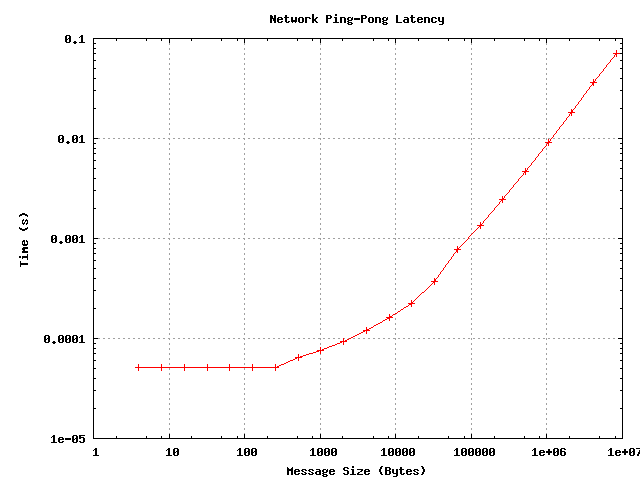
\includegraphics[width=0.99\textwidth]{pics/netplot.png}
	\end{center}%
	\caption{netplot.png
	}
	\label{fig: netplot}
\end{figure}%
%=================================================================

